the aim of this project is simulating the value of a random vector $X$ whose component random variables are dependent. Markov chain Monte Carlo (MCMC) method is a powerful approach for generating a vector whose distribution is approximately of $X$. MCMC comprise a class of algorithms for sampling from a probability distribution. By constructing a Markov chain that has the desired distribution as its equilibrium distribution, one can obtain a sample of the desired distribution by observing the chain after a number of steps. The more steps there are, the more closely the distribution of the sample matches the actual desired distribution.\\
\subsection{Metropolis-Hastings algorithm}
Metropolis–Hastings algorithm is a Markov chain Monte Carlo (MCMC) method for obtaining a sequence of random samples from a probability distribution from which direct sampling is difficult. This sequence can be used to approximate the distribution.

First part of this exercise, we generate Random Walk Metropolis-Hastings (RW-MH) Simulation of the Queue Problem.

\begin{center}
    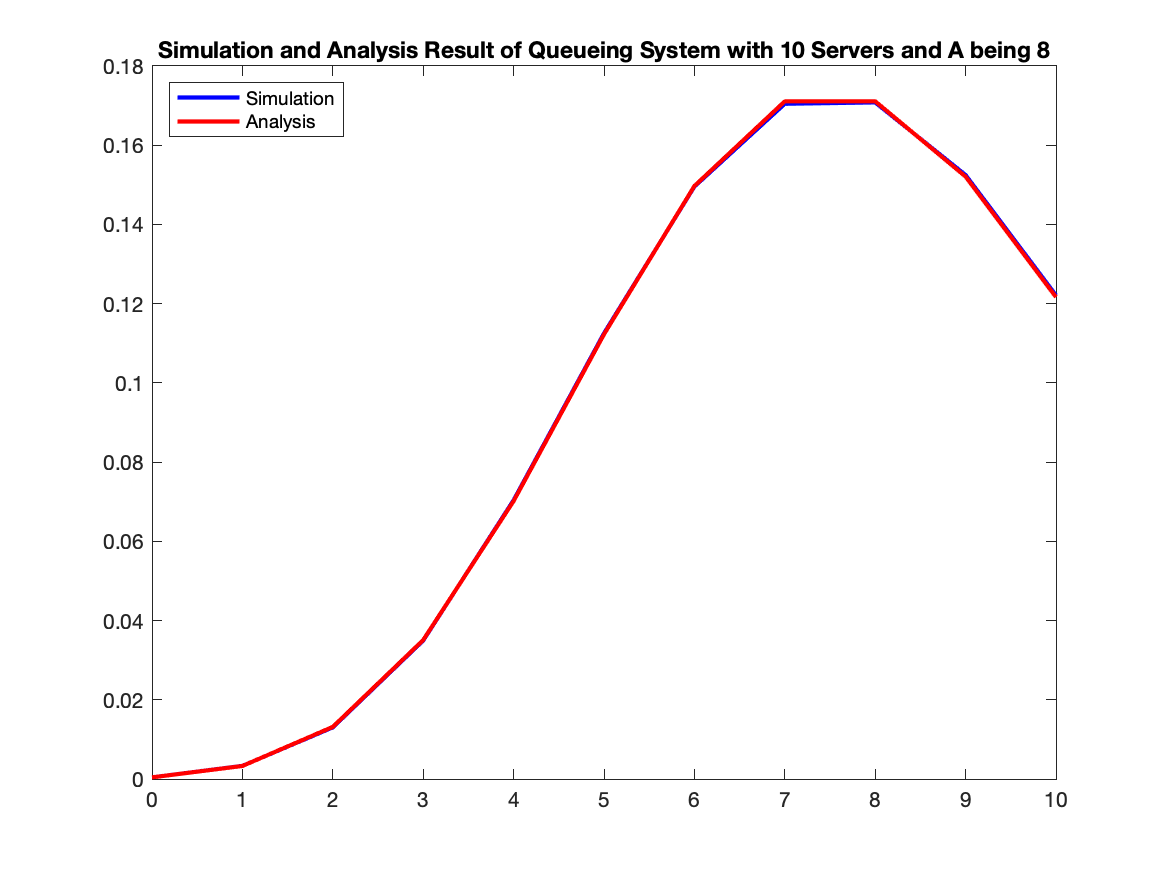
\includegraphics[scale=0.6]{Figures/figure6_1.png}\\
    \figuretitle{Figure 13: Simulation and analysis result of queuing system with 10 servers and A being 8.}
\end{center}

\subsection{Metropolis-hasting with two dimensional}
we want to use Metropolis-Hastings, directly and coordinate wise to generate variates from this distribution. we use $A1,A2 = 4$
and $n = 10$.

Figure 11 shows simulation and analysis result of generating values by Metropolis-Hastings algorithm in one dimensional.

\begin{center}
    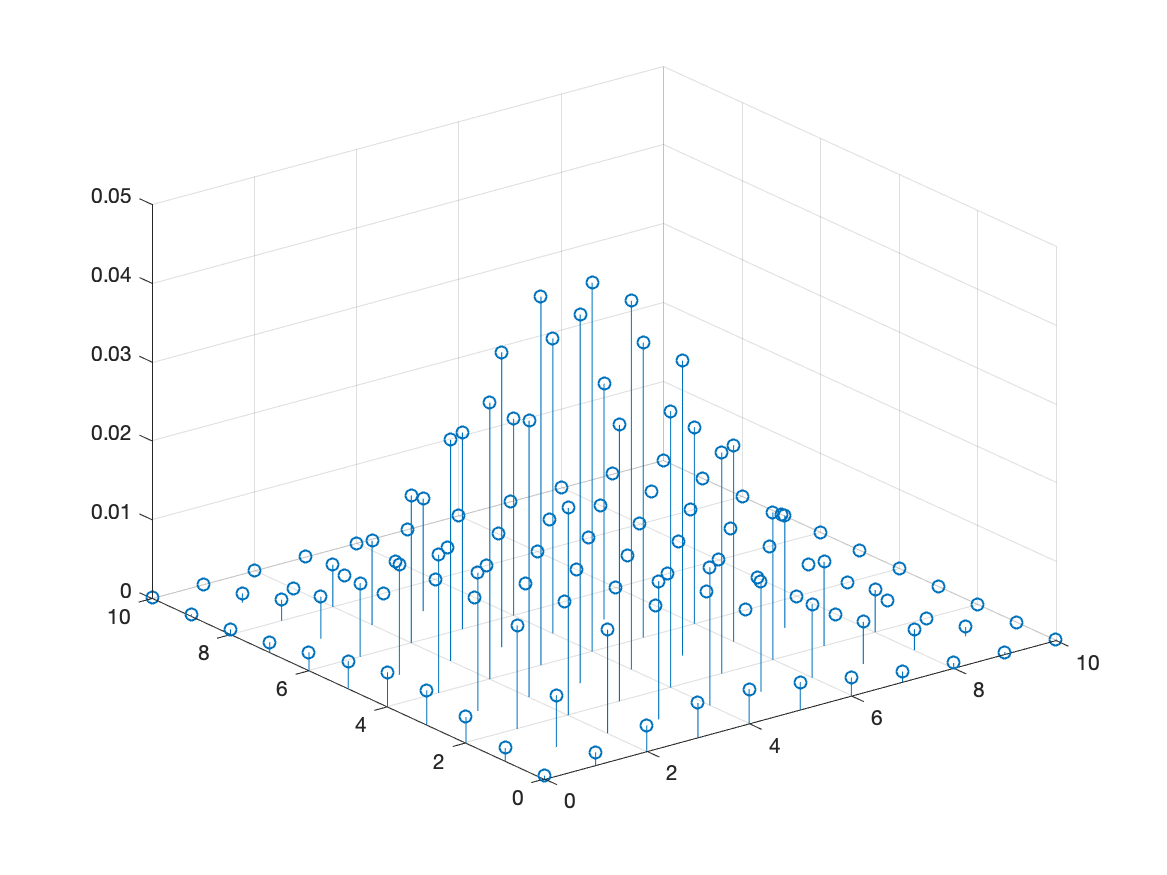
\includegraphics[scale=0.6]{Figures/figure6_2.png}\\
    \figuretitle{Figure 14: Analytical Result of Two-Dimension Problem.}
\end{center}

A algorithm for direct Metropolis-Hastings of two-dimension problem is implemented, which can be called "Array the 2-D Irregular Sample Space for 8-Direction Random Walk". The sample space like the following one is caused by the external conditions. So we have to find all the combinations in the sample space, and sort them randomly:

(0, 3) \\
(0, 2) (1, 2) \\
(0, 1) (1, 1) (2, 1) \\ 
(0, 0) (1, 0) (2, 0) (3, 0) \\

(0, 2) (0, 3) (2, 0) (3, 0) (1, 1) (0, 0) (2, 1) (1, 0) (1, 2) (0, 1)

Then, we array the sample space to rectangle, where we can perform two-dimension random walk. The head and tail of every column, row are connected respectively, so the random walk will not exceed the boundary:

(0, 2) (0, 3) (2, 0) (3, 0) (1, 1) \\ 
(0, 0) (2, 1) (1, 0) (1, 2) (0, 1)

The above illustration is a simple one, while this problem has 66 combinations in total in sample space. The effect of the random walk is shown in the following figure.

\begin{center}
    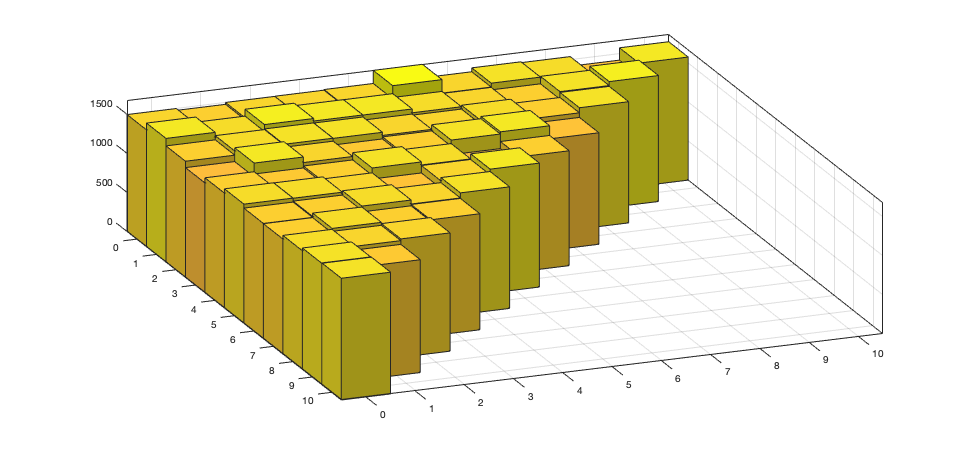
\includegraphics[scale=0.6]{Figures/figure6_7.png}\\
    \figuretitle{Figure 14: Direct Metropolis-Hastings of Two-Dimension Problem.}
\end{center}

Figures 15 and 16 present the generation of values by Metropolis-Hastings, directly and coordinate wise respectively. The red point the theoretical value. It can be seen that the algorithm works very well, and the statistical test result is shown in table 7.

\begin{center}
    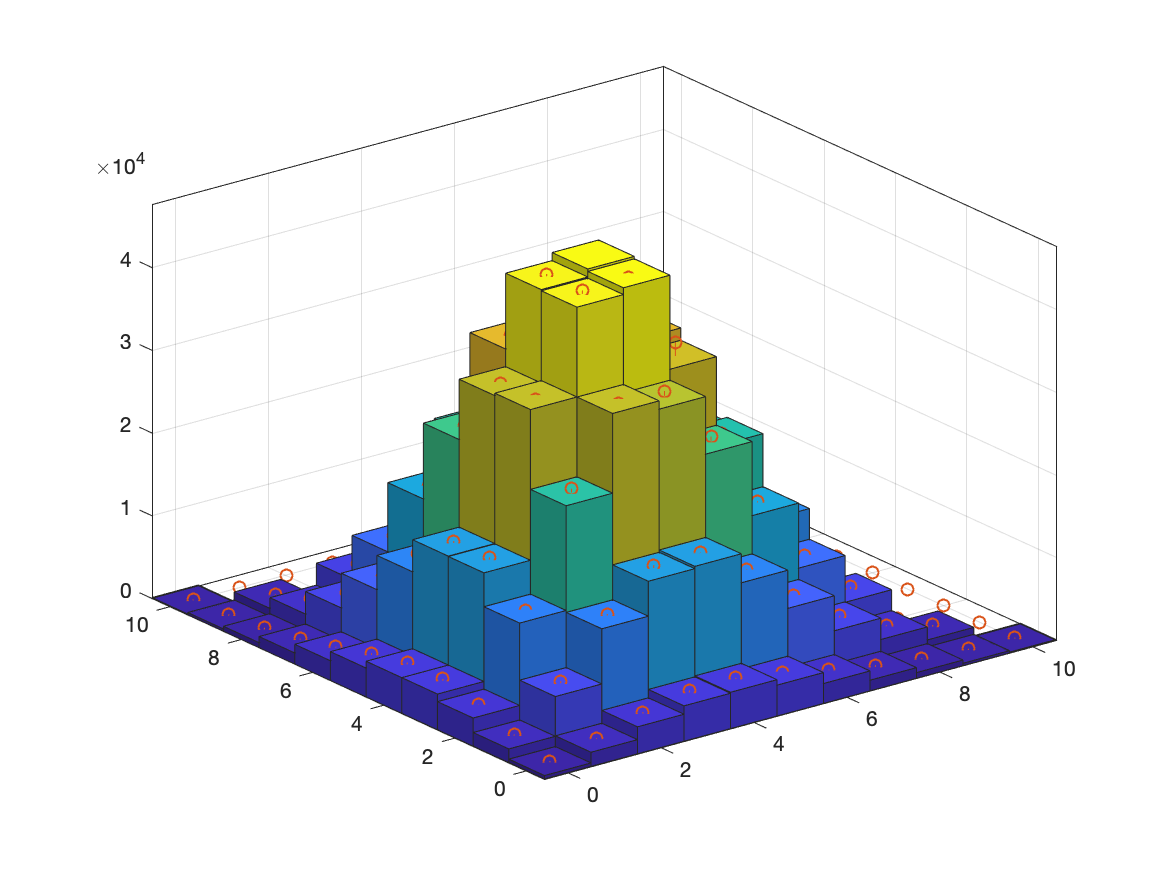
\includegraphics[scale=0.6]{Figures/figure6_3.png}\\
    \figuretitle{Figure 15: Direct Metropolis-Hastings of Two-Dimension Problem.}
\end{center}

\begin{center}
    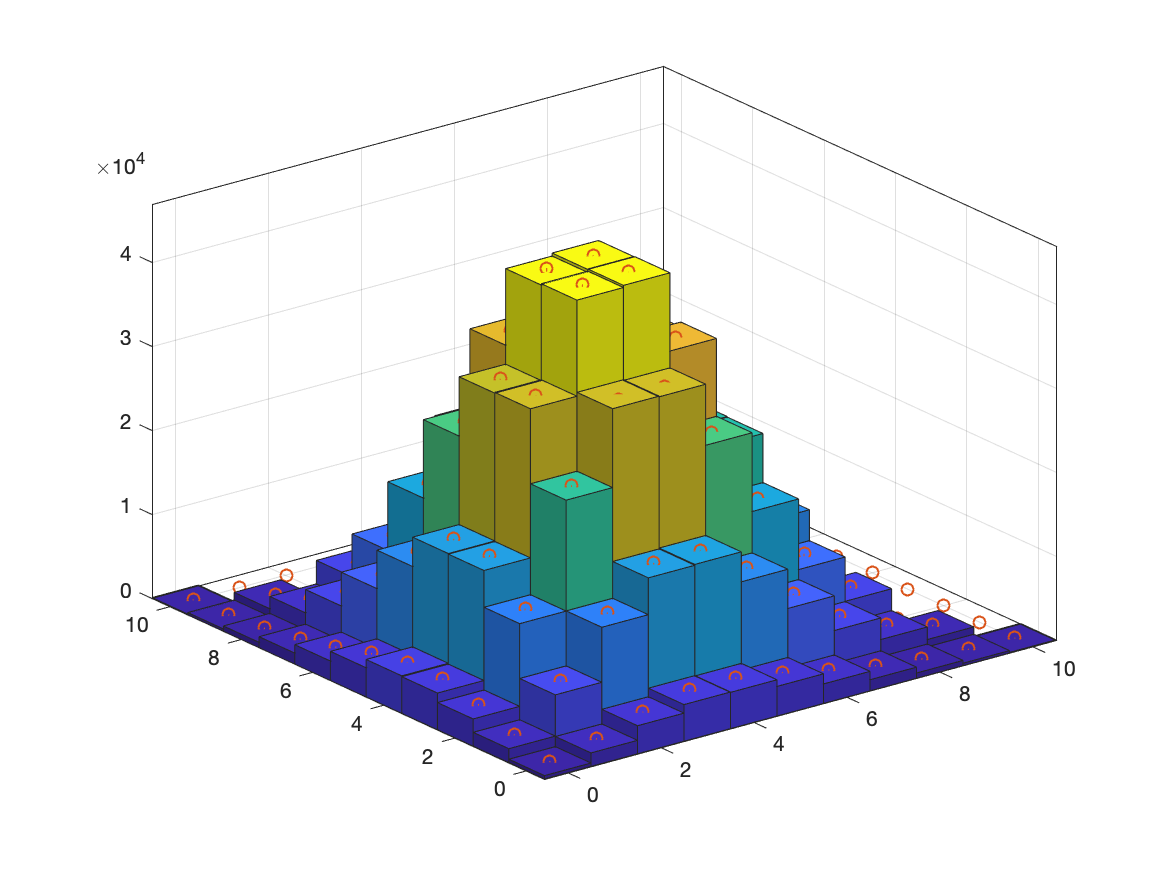
\includegraphics[scale=0.6]{Figures/figure6_4.png}\\
    \figuretitle{Figure 16: Coordinate-Wise Metropolis-Hastings of Two-Dimension Problem.}
\end{center}

\subsection{Gibbs sampling}
Gibbs sampling is a Markov chain Monte Carlo (MCMC) algorithm for obtaining a sequence of observations which are approximated from a specified multivariate probability distribution, when direct sampling is difficult. This sequence can be used to approximate the joint distribution or the marginal distribution of one of the variables.\\
The Gibbs sampling assumes for any $i,i=1,...,n$ and any values $x_j$, $j\neq i$, we can generate random variable $X$ having the probability mass function

\begin{equation}
    P\{X=x\} = P\{X_{i}=x|X_{j}=x_{j},j\neq i\}
\end{equation}

\begin{align}
    P(i, j) &= \frac{1}{K} \frac{A_1^i}{i !} \frac{A_2^j}{j !} = \frac{g(i, j)}{K} \qquad 0 \geq i + j \geq 10 \\
    P\{X=x\} &= P\{X_{i}=x|X_{j}=x_{j},j\neq i\} = \frac{P\{X_{i}=x, X_{j}=x_{j},j\neq i\}}{P\{X_{j}=x_{j},j\neq i\}} \\
    P\{X=x\} &= \frac{g(x, x_{j})}{\sum_{k = 0}^{10 - x_{j}} g(k, x_{j})} = \frac{A_1^x}{x !} L_{x_{j}} \qquad L_{x_{j}} =  \frac{ A_2^{x_{j}}}{ x_{j} ! \sum_{k = 0}^{10 - x_{j}} g(k, x_{j})} 
\end{align}

Figure 17 shows coordinate wise solution using Gibbs sampling.

\begin{center}
    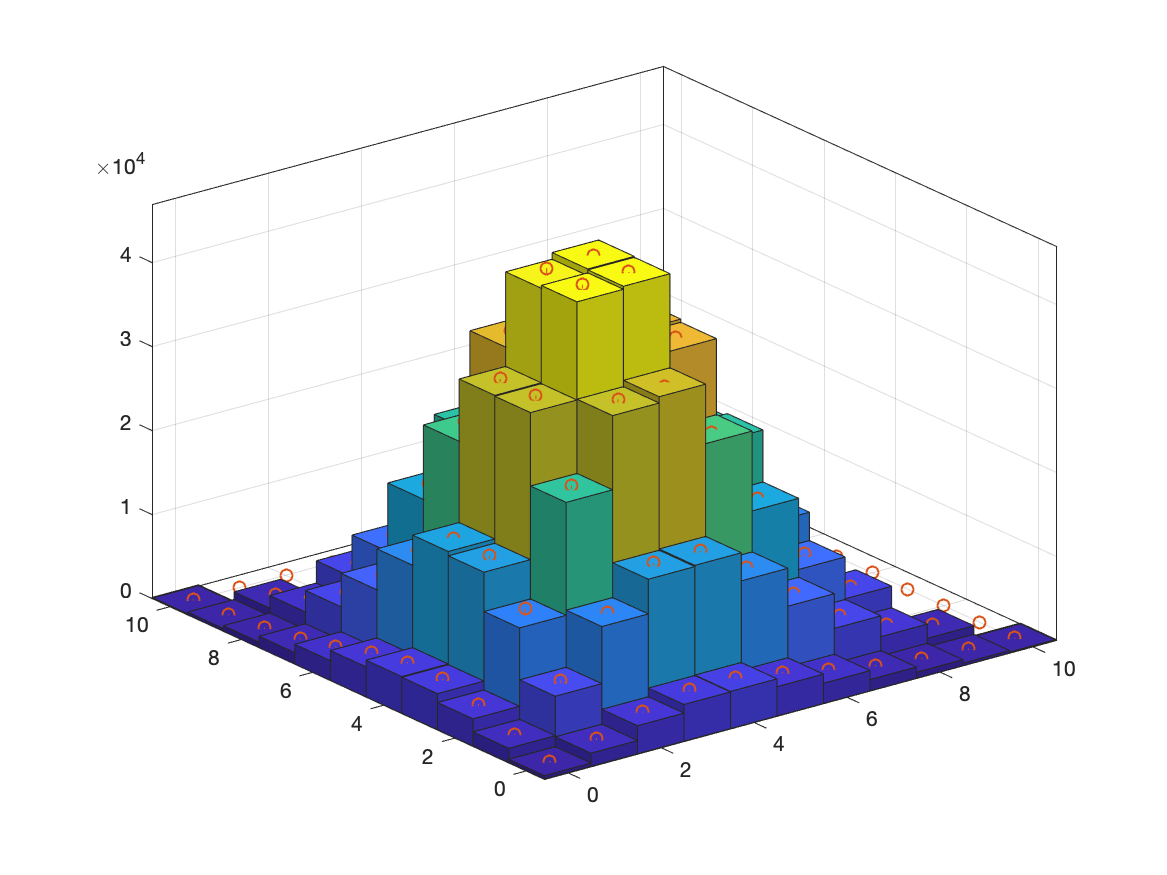
\includegraphics[scale=0.5]{Figures/figure6_5.png}\\
    \figuretitle{Figure 17:Coordinate wise Gibbs sampling .}
\end{center}\\
\\
Table 5 show $\chi^2$ values and Critical $ \chi^2$ values for 4 different methods.\\
\begin{center}
    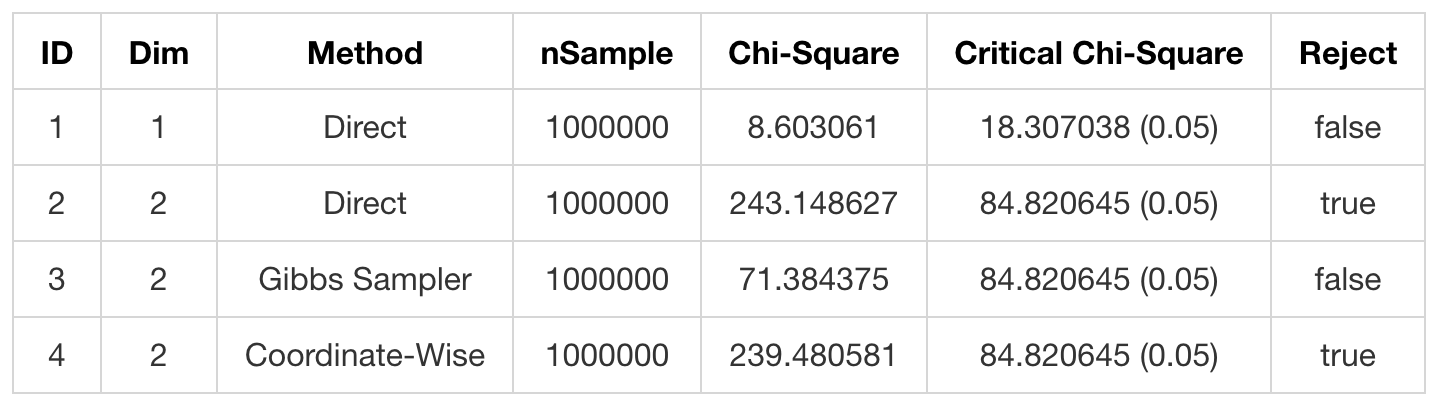
\includegraphics[scale=0.5]{Figures/figure6_6.png}\\
    \figuretitle{Table 7:results of $\chi^2$ Test for different methods .}
\end{center}\\